
\title{Demystify Visualiser}

\author{
       	Matthew J McIlree
}

\newcommand\demystify{\textsc{Demystify}\xspace}
\newcommand{\eprime}{\textsc{Essence Prime}\xspace}
\date{\today}

\documentclass[10pt]{article}
\usepackage{xspace}
\usepackage{graphicx}

\begin{document}
\maketitle

\section{Introduction}
The \demystify Visualiser is a single-page web application that makes the explanations and functionalities offered by \demystify more understandable and useful to end users. It uses React.js for a client-side interface, which communicates with a server-side API built using the Flask Python library. The JSON output produced by the \demystify command-line tool can be loaded and visualised with a graphical representation of the board and corresponding list of explanations. There is also the option to run the tool live on a server, without having it installed locally, enabling interactive choices from the user. 

\begin{figure}[h]
    \begin{center}
        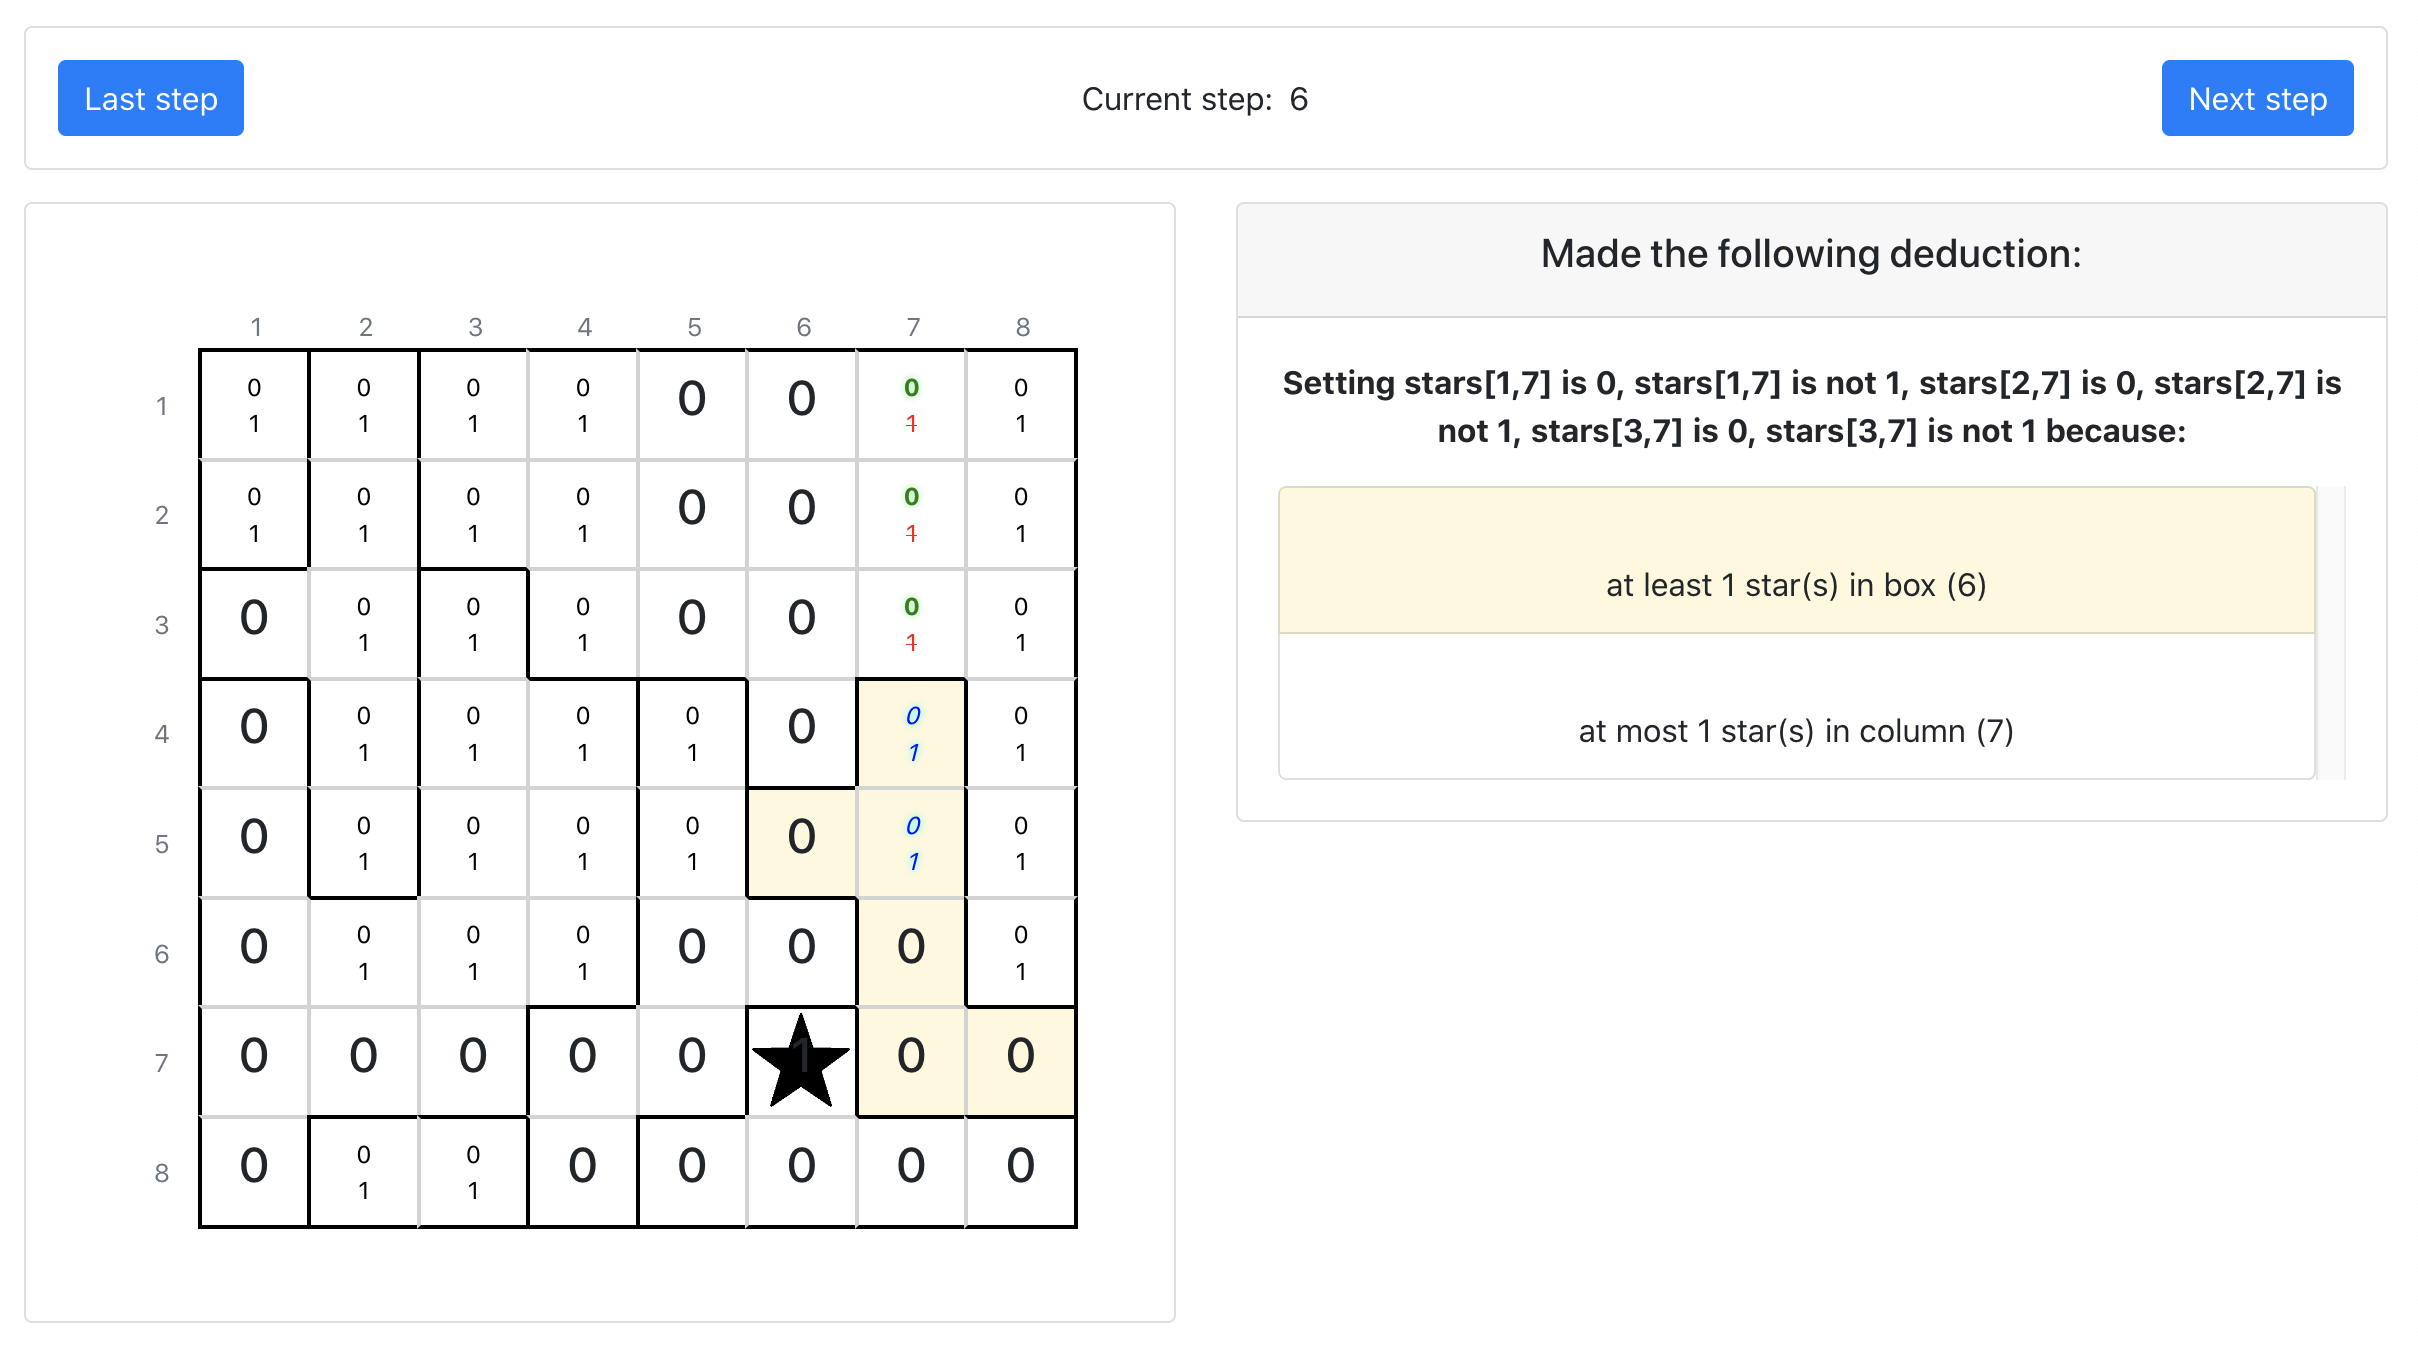
\includegraphics[width=\textwidth]{visualiser1}
    \end{center}
   \caption{ An explanation produced by \demystify, as displayed in the visualiser interface.}
\end{figure}

\section{Visualising Explanations}
To explain the solution to any particular puzzle \demystify produces a series of reasoning steps, sometimes combining simple deductions into a single step. The visualiser's primary function shows the user one reasoning step at a time. Each step has a representation of the puzzle state on the left, emphasising newly solved literals, and a scrolling list of the deductions made in English along with the reasons for those deductions on the right. 

For the purposes of this tool, all puzzle states are reduced to a grid of cells. A solved cell contains a single bold value, while an unsolved cell contains a sub-grid of possible values. The can be styled in a solving step to show how they are being used in a particular deduction: deduced true, deduced false, or involved in the reasoning. 
\begin{figure}[h]
    \begin{center}
    	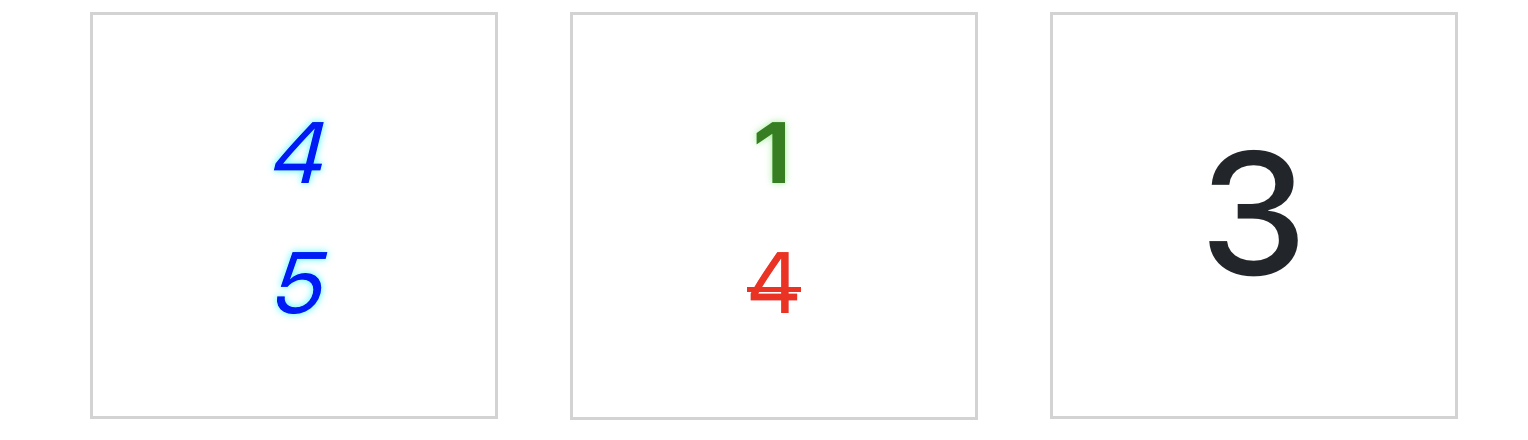
\includegraphics[width=0.6\textwidth]{visualiser2}
    \end{center}
    \caption{How the visualiser styles values in cells. From left to right we have a cell with involved values, a cell with a value deduced to be negative and a value deduced to be positive, and a cell with an already solved value.}
\end{figure}

In order to clarify the parts of the puzzle relevant to any particular reason for a deduction, the literals involved in the corresponding MUS can be highlighted as part of a two-way mouse-over effect. When a possible value is moused-over, all the reasons it is involved with are highlighted in the explanation list, and when an explanation is moused-over, all involved values on the grid are highlighted.

\section{Styling Puzzles}
A grid of numeric values along with the deductions in plain English is sufficient to represent \demystify's output, however, with many puzzles it is lacking some visual cues that would make an explanation more immediately understandable. These additional aspects include non-rectangular grid shapes, differing border thicknesses, pictures rather than numbers for solved values, and extra descriptors such as row and column sums. For most of the puzzles currently modelled for use by \demystify, the visualiser provides these additional puzzle styles. 

\begin{figure}[h]
    \begin{center}
    	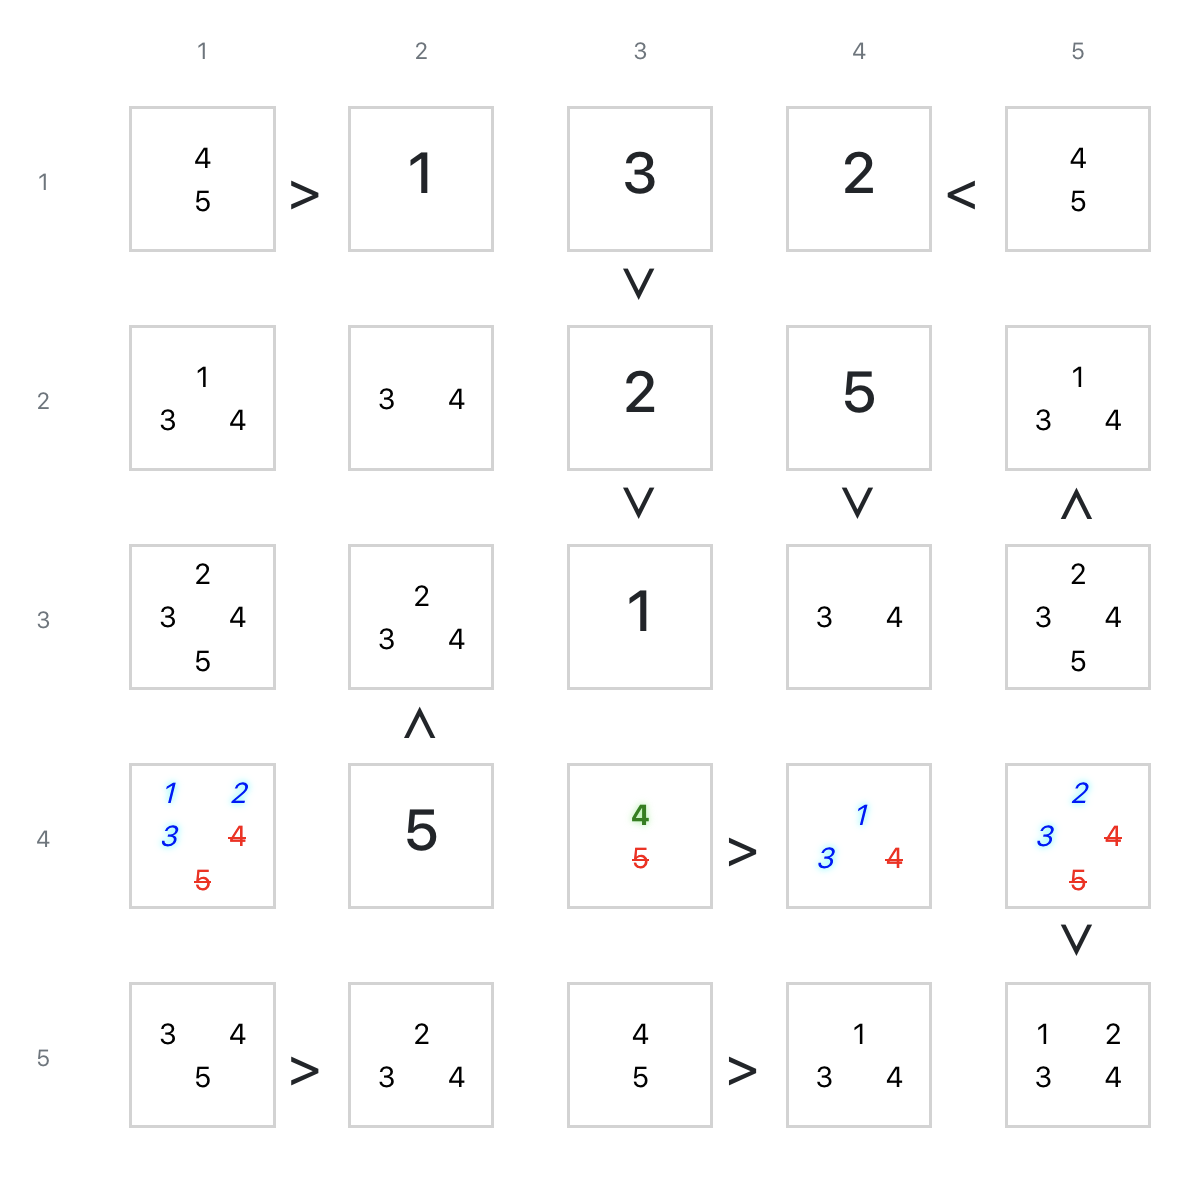
\includegraphics[width=0.3\textwidth]{futoshikiviz}
        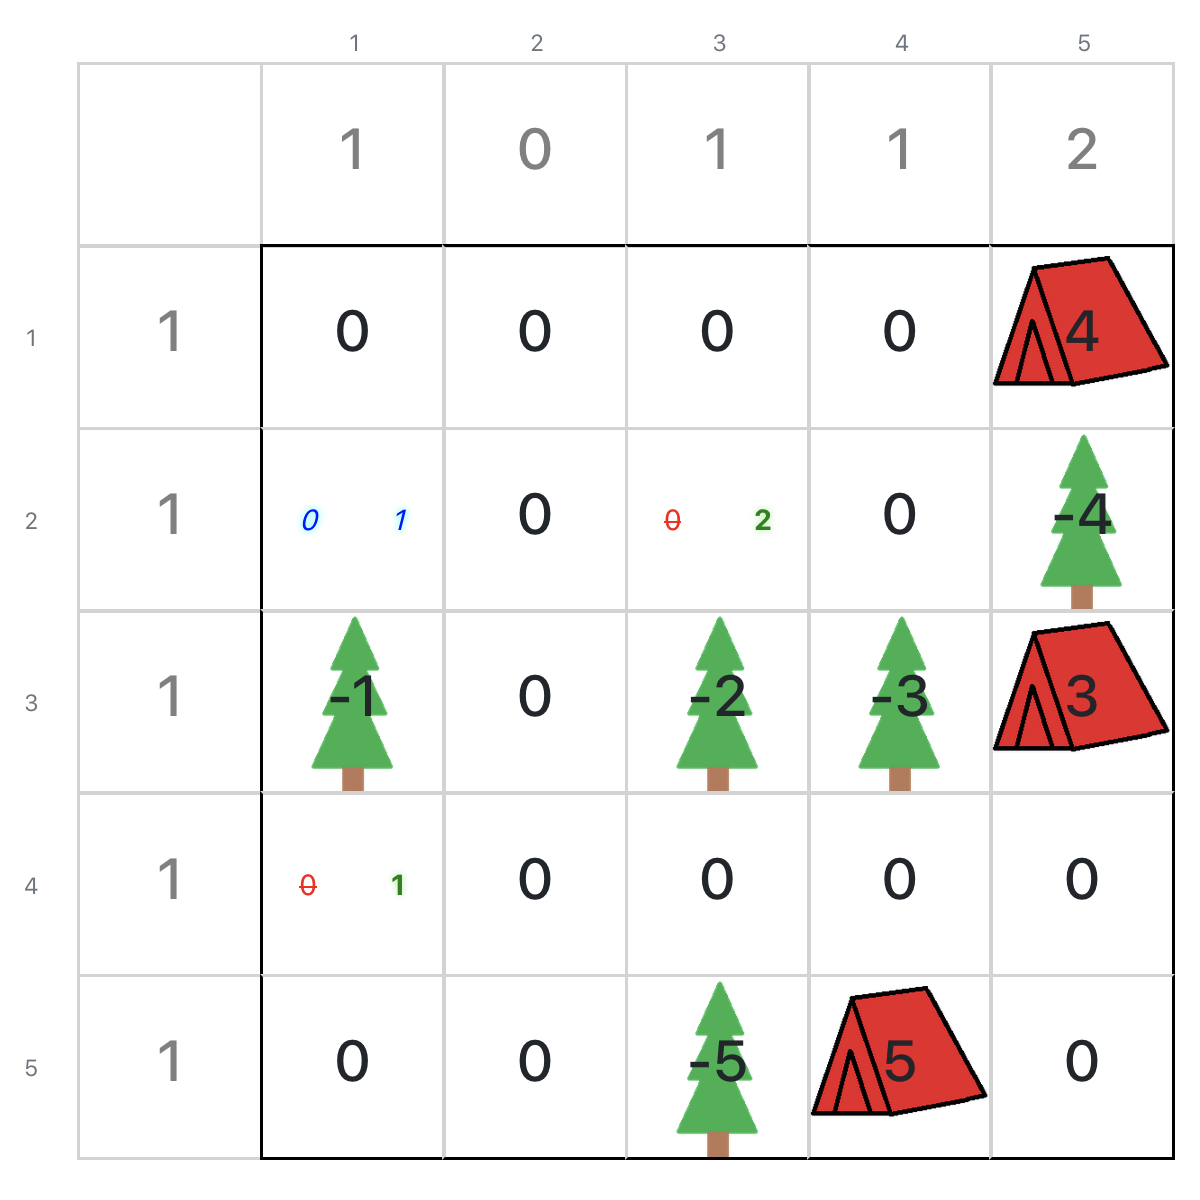
\includegraphics[width=0.3\textwidth]{tentsviz}
        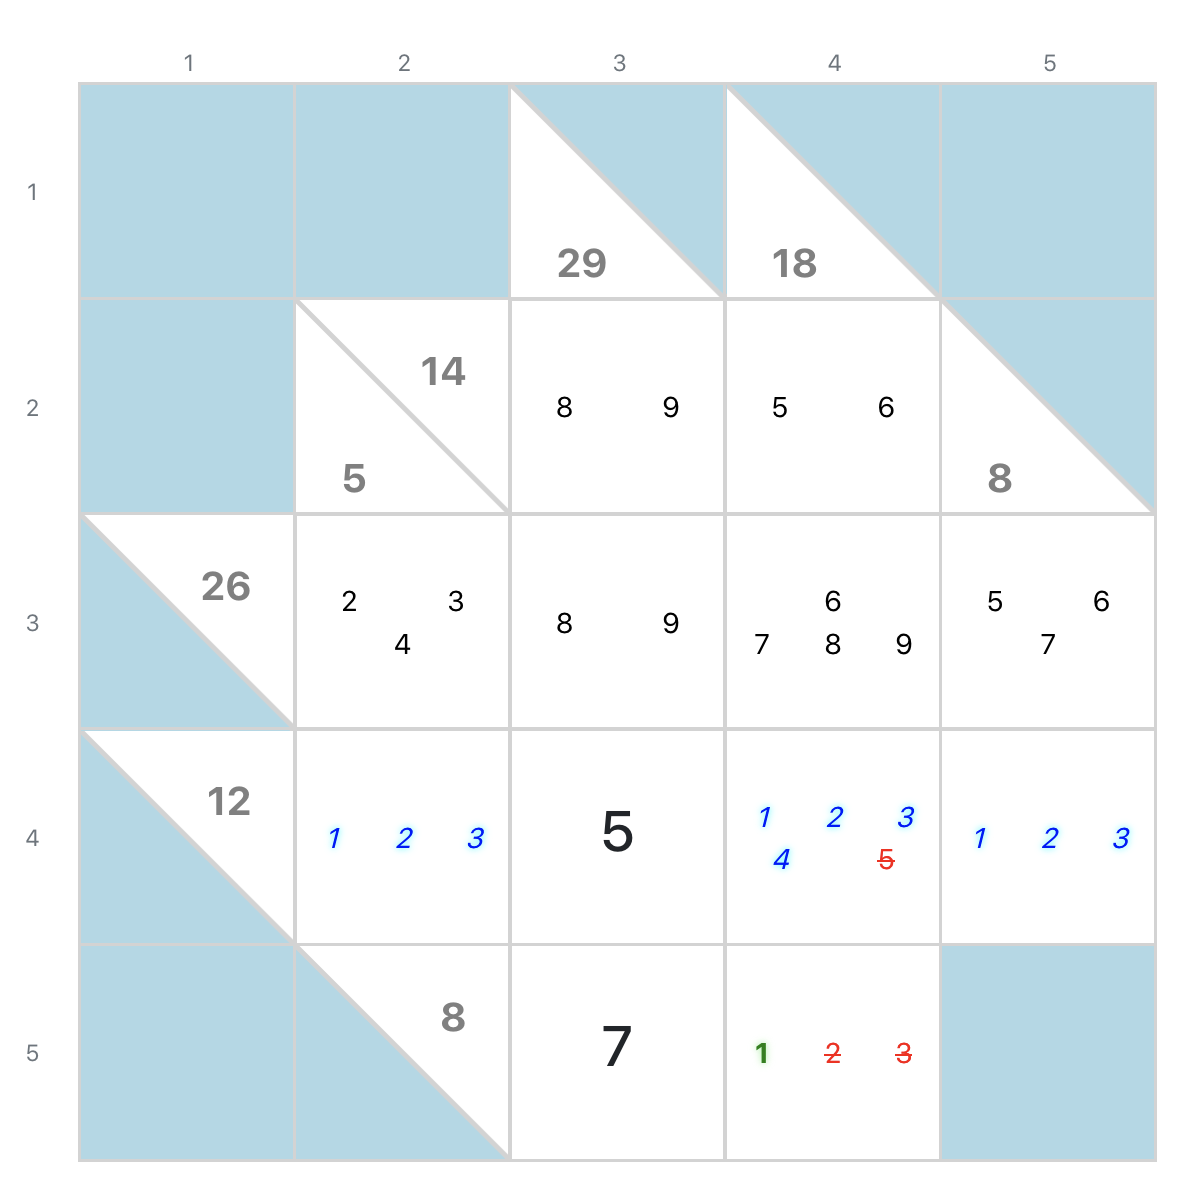
\includegraphics[width=0.3\textwidth]{kakuroviz}
    \end{center}
   \caption{ Some examples of the diversity of styles required for various puzzles. From left to right we have Futoshiki, Tents and Trees, and Kakuro.}
\end{figure}

This is achieved by creating a set of common properties of a puzzle grid that individual puzzle styles may want to alter, and implementing these with default values as part of a base `Board' component. \demystify includes the relevant properties of each puzzle, parsed from the \eprime description, in it's output, and so the task of creating a new puzzle visualisation is reduced to the task of writing a small wrapper class that translates the \demystify puzzle parameters into properties for the generic `Board'.
\\ \\
Properties currently available are:

\begin{itemize}
\item Borders for each cell
\item Extra inner borders for each cell
\item Background graphics for each cell
\item Background graphics to associate with certain solved values
\item Solved values to hide
\item Small numbers to display in the corners of cells
\item Label to display between cells
\item Space between cells
\item Extra rows and columns to append or prepend to the grid.
\end{itemize}

\section{Interactive Features}
The other significant feature of the visualiser application is the ability to run \demystify via a web API. This means that it is possible to make use of the tool without installing any of the dependent software, as well as facilitate user intervention in the solving process, allowing more influence over the final sequence of explanations.

Because the time taken to produce an outputs for different puzzles can vary significantly, the application implements a simple Job-Queue pattern using a Redis database and the RQ library to manage requests for \demystify tasks and polling for output. 

The user is able to upload their own \eprime input files, or select them from a predefined set, and then run \demystify in one of three modes. First, there is the default mode, where explanations for all steps of the puzzle solution are computed and passed to the visualisation. Secondly, there is a ``Choose MUSes manually" mode, where one step is sent to \demystify at a time, showing the visual interface between requests, and allowing the user to choose which MUS is used for the solution going forward if \demystify has found multiple options. Finally, there is the ``Force literal choices" mode, which allows the user to force demystify to produce an explanation for a particular literal, regardless of the associated MUS size. These interactive choices can be useful if the user wants to use \demystify to compare with their own solving techniques or solving techniques from other sources. 

Additionally, the application provides some other helpful features, such as the ability to build a Sudoku instance using an interface, and also to change the core MUS-finding algorithm used by \demystify.





\end{document}

